\documentclass[11pt]{article}
\usepackage[margin=2.5cm]{geometry}
\usepackage{graphicx}
\usepackage{booktabs}
\usepackage{amsmath}
\usepackage{amssymb}
\usepackage{parskip}
\usepackage{enumitem}

\title{Progress Update}
\author{Chalakon Pornjariyawatch \\ COMFHA Lab, Kasetsart University}
\date{November 6, 2026}

\begin{document}
\maketitle

\noindent\textit{Changes since the last update (September 25, 2026):}
\begin{itemize}[itemsep=2pt]
  \item \textbf{All BLG analyses now cover the full 1000 ns for every replica.} Surface
    tension for R1/R2/R3, the last 500~ns gap, is closed; $\gamma$ is unchanged
    qualitatively (51.9--52.3~mN/m, all four replicas).
  \item \textbf{Correction to previously reported CAS values.} The analysis selection
    had omitted the five phosphoserine residues (15, 17, 18, 19, 35); fixed and rerun.
    N-term SASA: CENTER 25.81 $\pm$ 2.39 (was 25.41 $\pm$ 1.97), R1 25.42 $\pm$ 1.45
    (was 24.77 $\pm$ 1.40) nm$^2$. DSSP coil: 69.8\% / 76.1\% (was 71.0\% / 76.6\%).
    Contact unchanged (99.5\%). Conclusions unchanged. BLG was not affected.
  \item \textbf{Accessible-feature SASA normalised for region size.} The $\sim$7-fold
    raw difference between CAS N-term (25 residues) and BLG calyx (9 residues) reported
    on September 25 is mostly a size effect. Per residue it is $\sim$2.7-fold, and as a
    fraction of each residue's own surface $\sim$2.6-fold (Table~2). CAS remains the more
    exposed, but the contrast is smaller than stated.
  \item \textbf{Figure 2 (structural dynamics) now complete for both proteins:}
    RMSD, RMSF and $R_g$, per replica.
\end{itemize}

\section*{BLG}

\begin{table}[h]
\centering
\small
\begin{tabular}{lcccc}
\toprule
Replica (1000 ns) & Calyx SASA (nm$^2$) & $R_g$ (nm) & $\gamma$ (mN/m) & Patch RMSD (nm) \\
\midrule
CENTER & 3.81 $\pm$ 0.46 & 1.504 $\pm$ 0.022 & 51.9 $\pm$ 0.5 & 0.198 $\pm$ 0.081 \\
R1     & 3.15 $\pm$ 0.34 & 1.497 $\pm$ 0.009 & 52.1 $\pm$ 0.4 & 0.347 $\pm$ 0.088 \\
R2     & 3.59 $\pm$ 0.32 & 1.494 $\pm$ 0.009 & 52.3 $\pm$ 0.2 & 0.254 $\pm$ 0.059 \\
R3     & 3.36 $\pm$ 0.48 & 1.507 $\pm$ 0.014 & 51.9 $\pm$ 0.5 & 0.276 $\pm$ 0.064 \\
\bottomrule
\end{tabular}
\caption{BLG per-replica summary, full 1000~ns each. $\gamma$ is given as mean $\pm$ block-averaged SEM (10 blocks of 100~ns);
the per-frame SD is $\sim$38~mN/m. For R1/R2/R3, $\gamma$ was previously 52.7/52.0/52.6~mN/m
from the first 500~ns only.}
\end{table}

\begin{table}[h]
\centering
\small
\begin{tabular}{lcccc}
\toprule
 & Region (residues) & Raw (nm$^2$) & Per residue (nm$^2$) & Exposed fraction$^\dagger$ \\
\midrule
BLG calyx (mean of 4 replicas) & 9  & 3.48  & 0.39 & 0.13 \\
CAS N-term (mean of 2 replicas) & 25 & 25.61 & 1.02 & 0.34 \\
CAS / BLG & & 7.4 & 2.7 & 2.6 \\
\bottomrule
\end{tabular}
\caption{Accessible-feature SASA, three normalisations. Computed on 401 frames
(every 5~ns) per replica. $^\dagger$Region SASA in the full protein divided by the sum of
each residue's SASA alone in the same frame. CAS values include the five
phosphoserines.}
\end{table}

\begin{figure}[h]
\centering
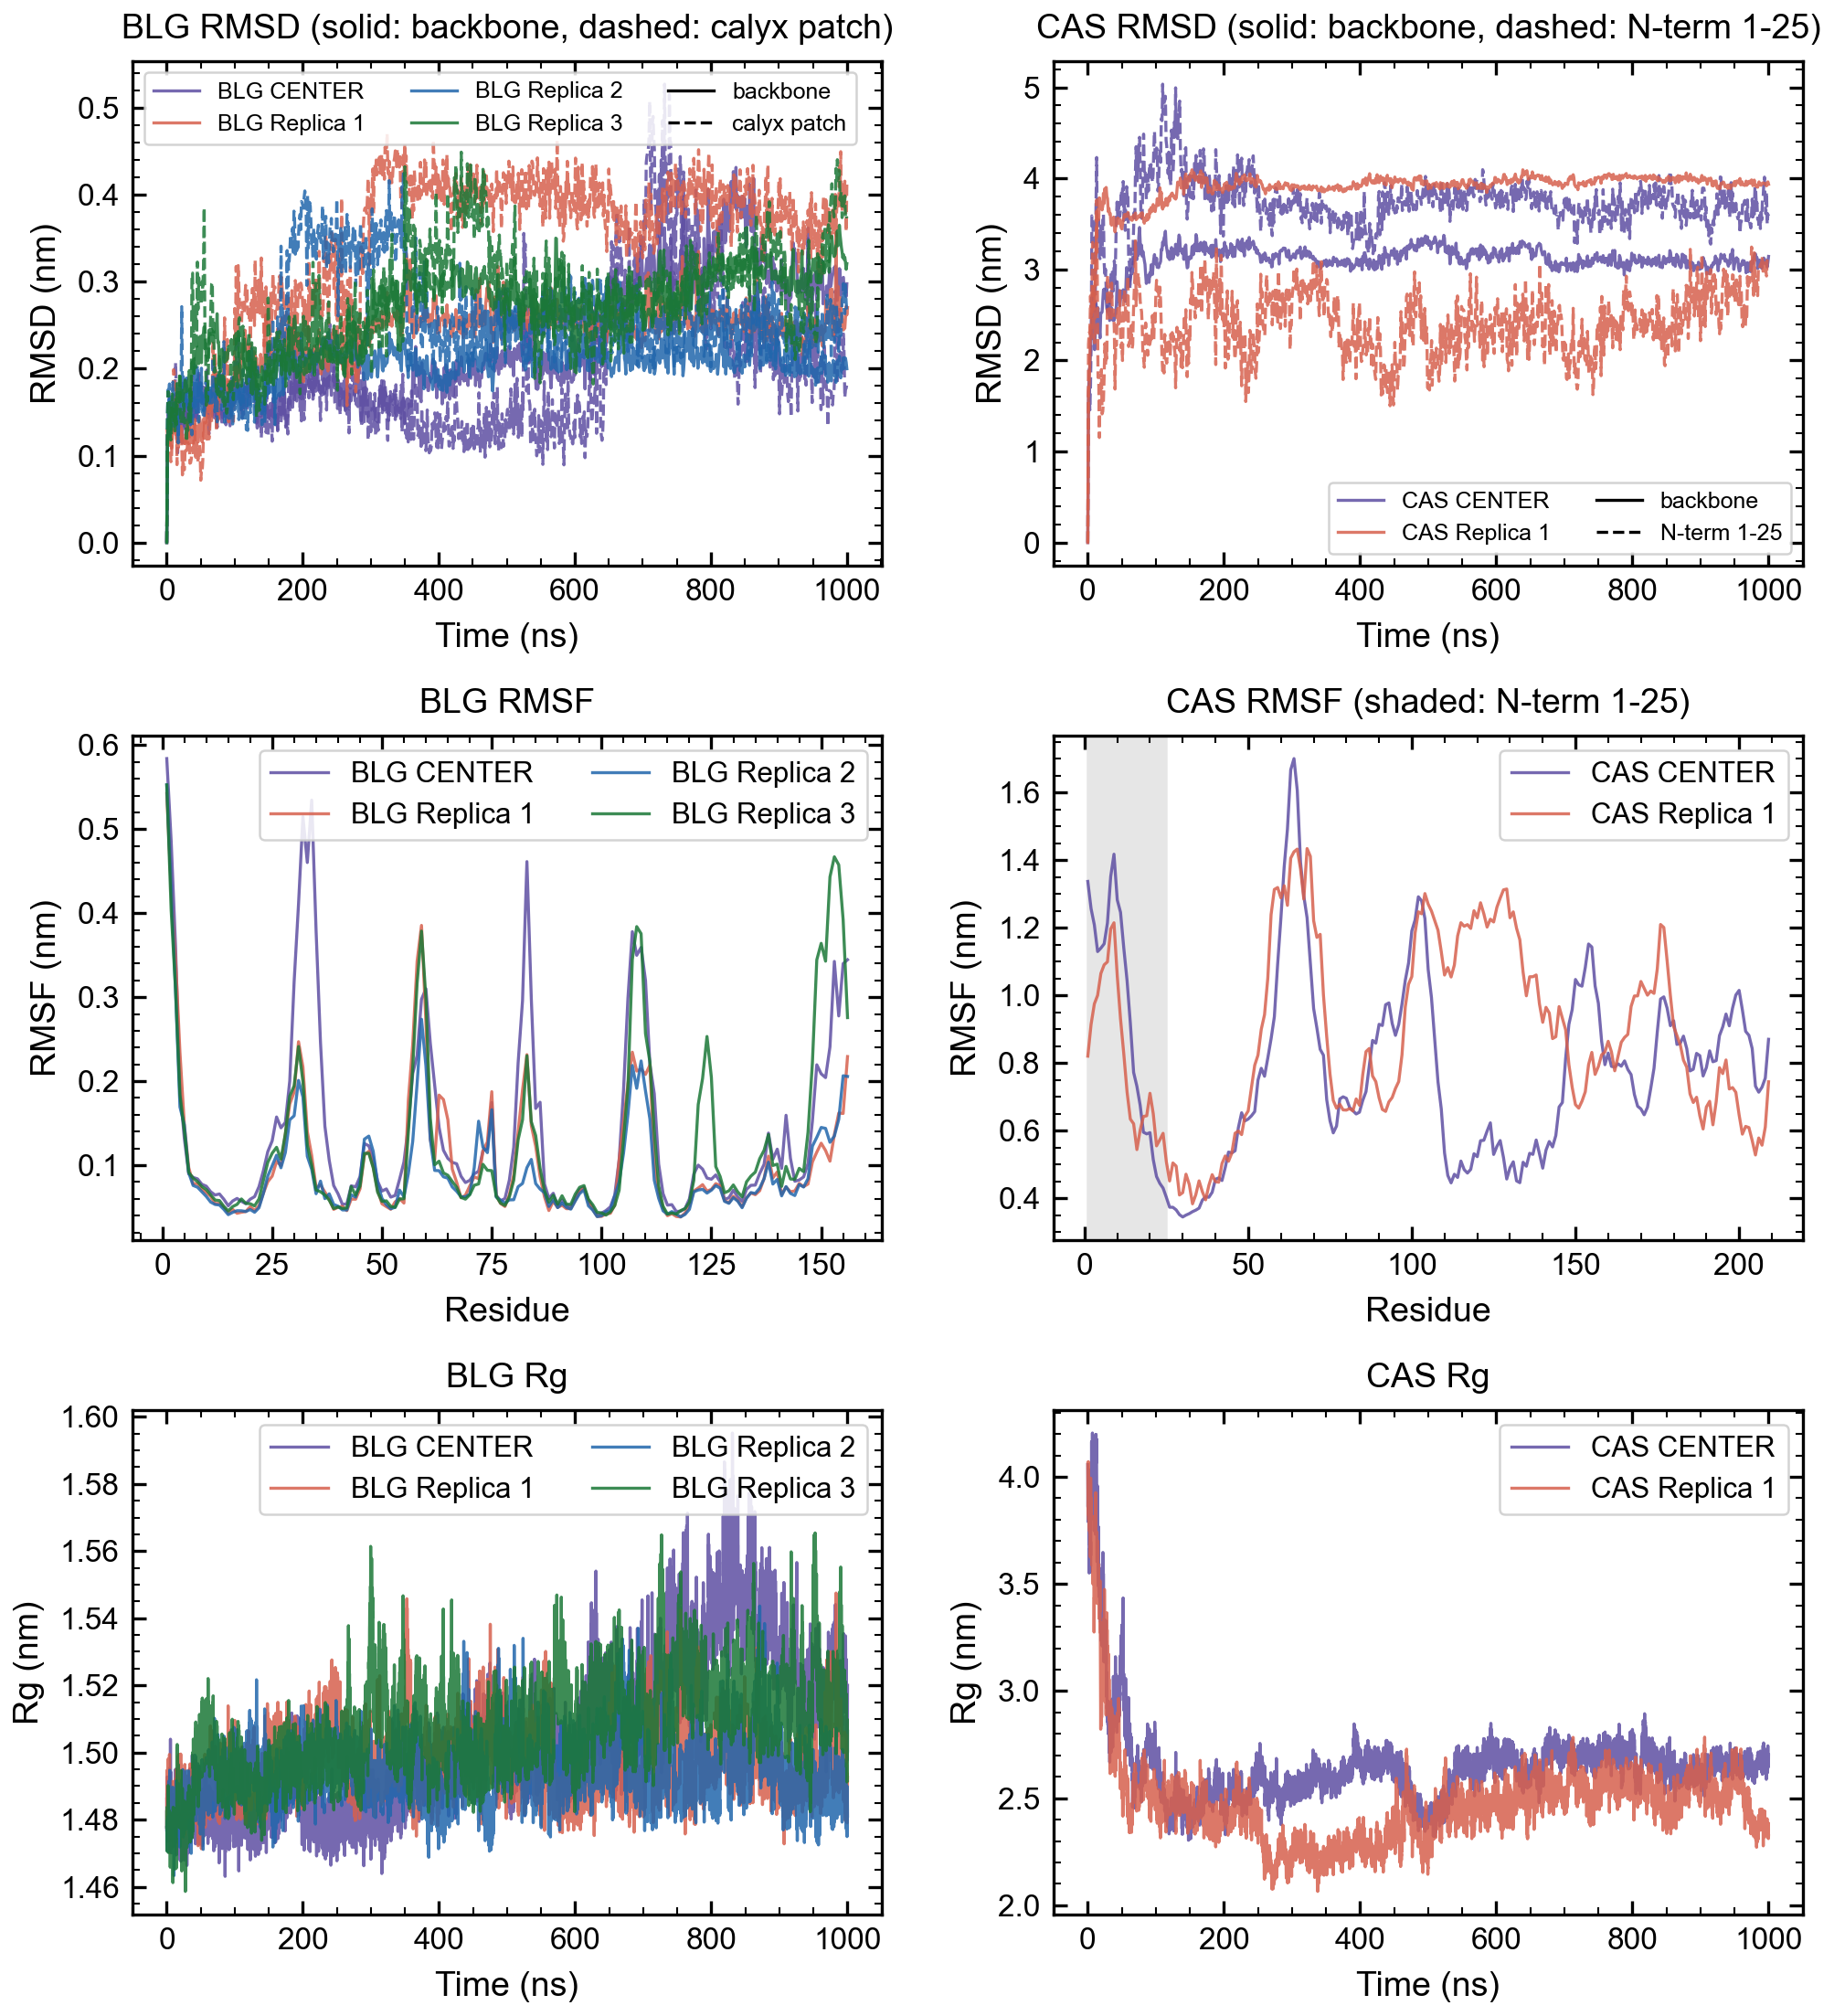
\includegraphics[width=0.8\textwidth]{../results/figures/paper/PAPER_FIG2_DYNAMICS.png}
\caption{Structural dynamics, per replica (not averaged). Left: BLG. Right: CAS.
Top: RMSD, backbone (solid) and calyx patch / N-term 1--25 (dashed). Middle:
per-residue RMSF. Bottom: radius of gyration. Axes differ between proteins; CAS is
disordered, so its RMSD/RMSF reflect chain mobility. R1 BLG's patch RMSD stays near
0.4~nm from $\sim$300~ns, after its longest contact event.}
\end{figure}

\end{document}
